\documentclass[aps,prl,preprint,superscriptaddress]{revtex4-2}

% You should use BibTeX and apsrev.bst for references
% Choosing a journal automatically selects the correct APS
% BibTeX style file (bst file), so only uncomment the line
% below if necessary.
%\bibliographystyle{apsrev4-2}
\usepackage{graphicx}
\usepackage{amsmath,amsthm,amssymb,mathtools}
\usepackage{amsfonts}
\usepackage{bm}
\usepackage{color}
\frenchspacing
%\graphicspath{/pics/}
%\graphicspath{{~/data/KannanLu/exp623/article/}}
\usepackage{listings}
\usepackage{color}
\definecolor{codegreen}{rgb}{0,0.6,0}
\definecolor{codegray}{rgb}{0.5,0.5,0.5}
\definecolor{codepurple}{rgb}{0.58,0,0.82}
\definecolor{backcolour}{rgb}{0.95,0.95,0.92}
% \definecolor{backcolour}{rgb}{0.18,0.18,0.18}
\lstdefinestyle{mystyle}{
    backgroundcolor=\color{backcolour},
    commentstyle=\color{codegreen},
    keywordstyle=\color{magenta},
    numberstyle=\tiny\color{codegray},
    stringstyle=\color{codepurple},
    basicstyle=\footnotesize,
    breakatwhitespace=false,
    breaklines=true,
    captionpos=b,
    keepspaces=true,
    numbers=left,
    numbersep=5pt,
    showspaces=false,
    showstringspaces=false,
    showtabs=false,
    tabsize=2
}
\lstset{style=mystyle}

\begin{document}

\title{Independent Component Analysis}

\author{Kannan Lu}
\author{Kittithat Krongchon}
\affiliation{Department of Physics, University of Illinois at Urbana-Champaign, Urbana, IL 61801, USA}

\date{\today}

\begin{abstract}
Indenpendent component analysis (ICA) is an unsupervised learning technique that is widely used in extracting independent factors in image, sound, and medical signals. In this document, we review the basic notions of the ICA including mathematical formulations and detailed algorithms. We also implement different algorithms based on higher-order statistics and information theoretic approaches. These algorithms are applied to sound signal disentanglement and electroencephalogram blinking signal removal with success.
\end{abstract}

\maketitle

\section{Introduction}
Independent component analysis (ICA) is one of the classical unsupervised learning techniques that is used to separate out latent variables or reduce dimensions. The motivation of the development of this technique is based on very commom problems. For instance, in reality, source signals are often corrupted with noise. In other words, data are composed of mutiple independent source signals. To isolate the signals from different sources, ICA can be a good choice. The famous example is the cocktail party problem, where the sound detectors record the superposition of various sound signals from different sources in the party. The goal is to separate out the observed signal into sounds from each different source. Since we do not know what the sources are and how these signals are mixed, this type of problem is called blind source separation (BSS) \cite{lee1998independent}. ICA is widely used in images, sounds, stock market, and medical signals, where latent independent variables are believed to exist. ICA can also be viewed as an extension of principal component analysis (PCA), where the latter maximizes the second order statistics (covariance matrix of data). ICA maximizes higher-order statistics or simply tries to look for independent components, not just uncorrelated components. In Fig.~\ref{fig:ICA_vs_PCA}, we show the ICA components $IC_{i}$ and PCA components $PC_{i}$ learned from the observed data $x_{i}$ with the original sources $s_{i}$ sampled from uniform distribution independently. Clearly, the ICA learned the independent components correctly, but the PCA did not in this case.


In this paper, we review mathematical background of the ICA technique, the detailed algorithm implementation and several realizations in typical examples.

\begin{figure}[b]
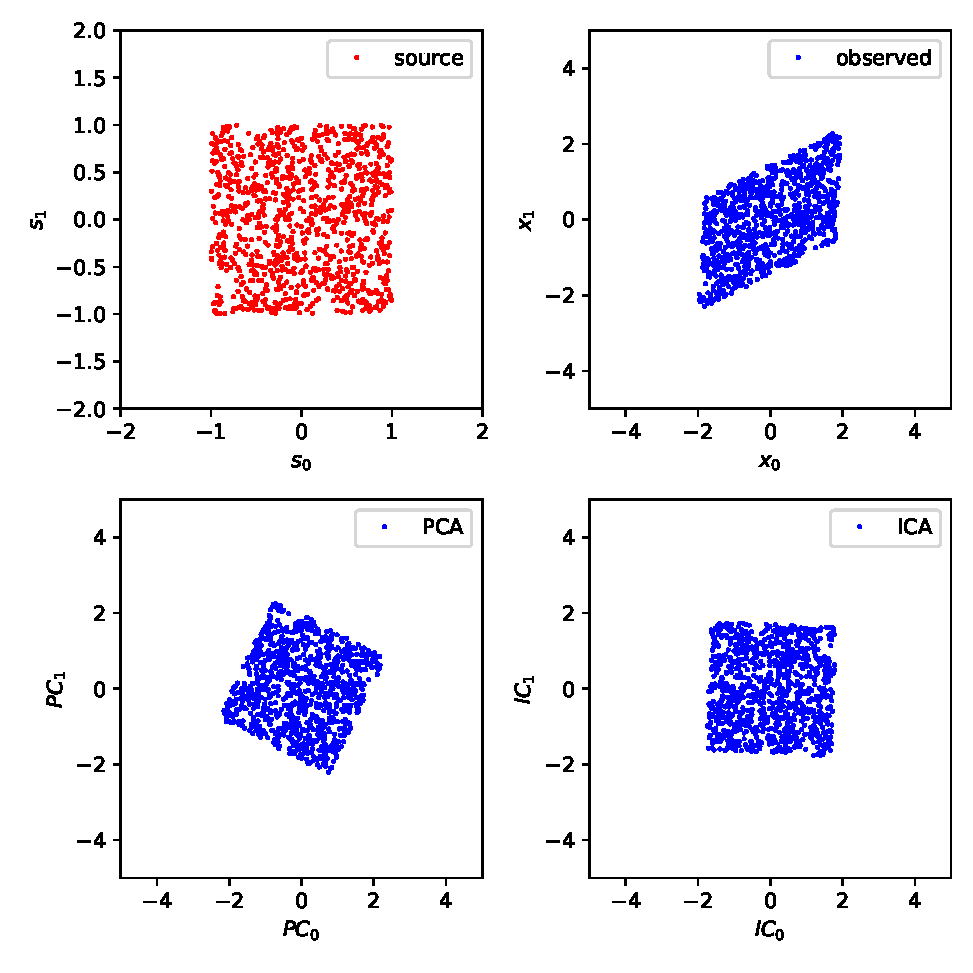
\includegraphics[width=0.8\textwidth]{scripts/ICA_vs_PCA.pdf}
\caption{\label{fig:ICA_vs_PCA} shows the PCA and ICA result of unmixing the observed data $x_{i}$ generated from two independent uniform variables $s_{i}$. The algorithm is based on maximizing the higher order moments. }
\end{figure}


\section{Mathematical Background}
\subsection{Definition of the problem and notations}
Before we delve into the detailed mathematical formalism, we first define the notations that we use throughout the whole document. We use boldface capital letters $\bf{A}$ for matrices, boldface lowercase letters $\bf{a}$ for vectors and ordinary lower case letters $a$ for scalars. We use subscripts to denote the components of matrices (i.e. $A_{ij})$ and vectors (i.e. $a_{i}$). Notice that these letters are not in boldface as they mean the specific component, which is just a scalar in $ \rm I\!R$. Superscripts are reserved for indexing different samples. For instance, $m$ samples of vector $\bf{a}$ can be denoted as $\bf{a}$$^{(k)}$ where $k = 1, 2, \ldots, m$. Following these conventions, we denote the original signal to be $\bf{s}$$^{(i)} \in \rm I\!R^{d}$. We consider the standard setting where the $d$ dimensional signals $\bf{s}$$^{(i)} \in \rm I\!R^{d}$ ($d$ original sources) are mixed and observed by $d$ detectors $\bf{x}$$^{(i)} \in \rm I\!R^{d}$ (i.e. the cocktail party scenario). That is there is a linear map between the $\bf{s}$$^{(i)}$ and $\bf{x}$$^{(i)}$, $\bf{x}$$^{(i)}$ $=$ $\bf{A}$$\bf{s}$$^{(i)}$, where $\bf{A} \in \rm I\!R^{d\times d}$ is known as the mixing matrix. The whole idea of ICA is to learn the inverse of the mixing matrix $\bf{W} = \bf{A}$$^{-1}$ from the observed data $\bf{x}$$^{(i)}$, known as the unmixing process. The learned independent components are denoted by $\bf{u} = \bf{W}\bf{x}$. This can be done in several different ways based on ideas of separating non-Gaussian signals and the original signals being independent. We will in this section discuss various mathematical formulations. All these various theoretical frameworks are constrained by the following conditions~\cite{lee1998independent}.
\begin{enumerate}
\item The number of sensors is larger than number of sources. This ensures that the mixing matrix is full rank.
\item The sources at each sample (time) are mutually independent.
\item At most one source is normally distributed.
\end{enumerate}
Without these conditions, the BSS problem is ill-defined. For simplicity, we will also restrict the discussion to cases where the number of detectors and sources are the same.
However, a generalization to the first condition is feasible, and the algorithms discussed in the following sections will still work.

Based on these definitions, we need to talk about some ambiguities embedded in the symmetry of the problem and justify that if the original signals are all Gaussians, they cannot be learned through the unmixing. There are two ambiguities that usually do not affect the practical application, namely the permutation ambiguity and the scaling ambiguity. It is trivial to see that the ordering of the original sources \{$s_{j}$\} is ambiguous.
In the case of scaling, if the original signal $\bf{s}$ is scaled by a non-zero constant to be $c\bf{s}$ where $c \neq 0$, then the mixing matrix $\bf{A}$ can be scaled by $1/c$ and will result in the same observed data $\bf{x}$$ = \frac{1}{c}\bf{A}$$c\bf{s}$. This scaling ambiguity can be further extended to each component of the original signal.
That is, for a particular component $j$, if we scale the component by $c_{j}$, the corresponding column of the mixing matrix can be scaled by $1/c_{j}$ to have the observed data unchanged (i.e. $x_{i} = \sum_{j}\frac{1}{c_{j}}A_{ij}c_{j}s_{j}$) \cite{ng_cs229}.

The other ambiguity that matters for the practical application is that the original sources cannot all be distributed as Gaussians \cite{lee1998independent, ng_cs229}.
To be more precise, in order to separate the independent components, we require that the original signals have at most only one component to be sampled from a Gaussian distribution, i.e. $s_{j}$ $\sim \mathcal{N}(\mu,\,\sigma^{2})$ for at most one $j$. Let's consider the case when all the original independent signals are Gaussians. That is, $s_{j}$ $\sim \mathcal{N}(\mu_{j},\,\sigma_{j}^{2})$ for $j = 1, 2, \ldots, d$.
Then, given the mixing matrix $\bf{A}$, we have
\begin{equation}
\mathbb{E}[\mathbf{x}] = \mathbf{A}\mathbb{E}[\mathbf{s}] = \mathbf{A}\bm{\mu}
\end{equation}
and
\begin{equation}
\mathrm{Cov}[\mathbf{x}] = \mathbb{E}[\mathbf{As}\mathbf{s}^t\mathbf{A}^{t}]-\mathbb{E}[\mathbf{As}]\mathbb{E}[(\mathbf{As})^{t}] =  \mathbf{A}\bm{\Sigma}\mathbf{A}^{t}-\mathbf{A}\mathbf{M}\mathbf{A}^{t},
\end{equation} where $\mathbf{M}$ and $\bm{\Sigma}$ are diagonal matrices of $\rm I\!R^{d\times d}$ with diagonal elements to be \{$\mu_{j}^{2}$\} and \{$\sigma_{j}^{2}$\}, respectively.
Due to the scaling ambiguity, this is the same as considering normally distributed signals with unity variance. Since each column $j$ of the mixing matrix $\mathbf{A}$ can be scaled by $\sigma_{j}$, $\tilde{\mathbf{A}}_{:j} = \sigma_{j}\mathbf{A}_{:j}$, and correspondingly, the signal needs to be scaled by $1/\sigma_{j}$, $\tilde{s_{j}} = \frac{s_{j}-\mu_{j}}{\sigma_{j}}$. Then,
\begin{equation}
\mathrm{Cov}[\mathbf{x}] = \tilde{\mathbf{A}}\mathbf{I}_{d\times d}\tilde{\mathbf{A}}^{t}.
\end{equation}
Now, if we consider a rotation $\mathbf{R} \in O(d)$ acting on the scaled source signals $\mathbf{\tilde{s}}$, the mixing matrix then changes to $\tilde{\mathbf{A}}\mathbf{R}$.
Upon this rotation, we would observe $\mathbf{x'}$ as $\mathbf{x'} = \tilde{\mathbf{A}}\mathbf{R}\tilde{\mathbf{s}}$, and $\mathbf{x'}$ is again normally distributed and has covariance matrix,
\begin{equation}
\mathrm{Cov}[\mathbf{x'}] = \tilde{\mathbf{A}}\mathbf{R}\mathbf{I}_{d\times d}\mathbf{R}^{t}\tilde{\mathbf{A}}^{t} = \tilde{\mathbf{A}}\mathbf{I}_{d\times d}\tilde{\mathbf{A}}^{t}.
\end{equation} This simply means that whether the sources are rotated or not the observed data will be distributed as $\mathcal{N}(0, \tilde{\mathbf{A}}\tilde{\mathbf{A}}^{t})$. Thus, because of the rotational symmetry of the multivariate Gaussian distribution, we cannot separate and obtain the original source signals. These derivations also indicate that given the observed data $\bf{x}$, we can whiten (apply PCA rotation and normalize each principal component) the data, and it does not affect the separated signals (up to scalings and mean translations). We will assume the observed data $\bf{x}$ are whitened if not explicitly stated in later discussions. That is $\tilde{\mathbf{x}} = \mathbf{K}(\mathbf{x}-\bm{\mu})$, where $\mathbf{K}$ is the whitening transformation. Then, to recover the source signals, we need to find $\mathbf{W}$ with orthonormal rows \{$\mathbf{w}_{i}^{t}$\} such that $\mathbf{s} = \mathbf{W}\mathbf{K}\mathbf{x}$.

\subsection{Higher order statistics approach}

The non-Gaussianity directly provides us with the methodologies used in finding the independent component. Notice that the PCA only finds the uncorrelated components but not necessarily independent. The ICA tries to find independent components where the joint distributions can be factorized into marginal distributions by investigating higher-order moments. There are multiple moment-based objective functions that have been used along the development of ICA. We define some of the notations and discuss one of the moment-based objective functions in detail.

As we discussed previously, we whiten the observed signals and we denote the whitened observed data as $\bf{x}$. The kurtosis and excess kurtosis of whitened variable $x$ are defined as
\begin{align}
\beta(x) := \mathbb{E}[x^{4}],~\kappa(x) := \beta(x)-3.
\end{align}
The standard normal random variable has excess kurtosis to be 0. When excess kurtosis $\kappa(x) < 0$, $x$ is said to be sub-Gaussian (flat around the center, e.g. uniform distribution). When $\kappa(x) > 0$, $x$ is super-Gaussian (heavy tail and sharp peak around the center, e.g. Laplace distribution).
The objective function to maximize can be $|\kappa(x)|$ and $\kappa^{2}(x)$ etc. This is further backed up by the following inequalities \cite{miettinen2015fourth}.
\begin{align}
\forall i \in \{1, \ldots, d\}, ~|\kappa(\mathbf{w}_{i}^{t}\mathbf{x})| &\leq \mathrm{max}\{|\kappa(z_1)|, \ldots ,|\kappa(z_d)|\}. \\
|\kappa(\mathbf{w}_{1}^{t}\mathbf{x})|+ \cdots + |\kappa(\mathbf{w}_{d}^{t}\mathbf{x})| &\leq |\kappa(z_1)|+ \cdots +|\kappa(z_d)|,
\end{align}
where $z_{i}$'s are the standardized independent components.

Thus, the problem is equivalent to finding an orthogonal transformation $\mathbf{W}$ with orthonormal rows \{$\mathbf{w}_{i}^{t}$\} such that the objective function can be maximized. In the case of the objective function $L(\mathbf{w}) = |\kappa(\mathbf{w}^{t}\mathbf{x})|$, this amounts to iterating the $\mathbf{w}$ with gradient~\cite{hyvarinen2000independent},
\begin{equation}
\frac{\partial |\kappa(\mathbf{w}^{t}\mathbf{x})|}{\partial \mathbf{w}} = 4~\mathrm{sign} [\kappa(\mathbf{w}^{t}\mathbf{x})]\{\mathbb{E}[\mathbf{x}(\mathbf{w}^{t}\mathbf{x})^{3}]-3\mathbf{w}||\mathbf{w}||^{2}\}.
\end{equation}
This objective function captures both sub-Gaussian and super-Gaussian distributions for the source signals but the kurtosis is sensitive to the outliers of the observed data. Hence, some adaptive objective functions are used in practice more extensively based on negentropy~\cite{hyvarinen2000independent}.

\subsection{Information theoretic approach}

Apart from the moment-based approaches, there are several information theoretic methods. In this section, we will review all different information theoretic frameworks and show that essentially they are equivalent. Then we will talk about the learning rules for these theoretical formulations in the subsequent section.
The centralized quantity in this formalism is the mutual information, which is defined as the Kullback--Leibler (KL) divergence of the multivariate distribution of the observed data $\bf{x}$ and product of all its marginal distributions, i.e.
\begin{equation}
I(\mathbf{x}) = \sum_{\mathbf{x}}p(\mathbf{x})\log\frac{p(\mathbf{x})}{\prod_{i}p_{i}(x_{i})}.
\end{equation} $I(\bf{x})$ is non-negative and is zero if and only if the $\bf{x}$ are independent. Several different information theoretic approaches have been formulated in history and can be unified in the concept of minimizing the mutual information of the separated components $\bf{u} = \bf{W}\bf{x}$.

One formulation in neural networks is to maximize information between inputs $\mathbf{x}$ and outputs $\mathbf{y}$, which implies that the output distributions are factorized and thus minimize the mutual information in the outputs $\mathbf{y}$.
Maximizing the information between inputs and outputs is to maximize the output joint entropy $H(\mathbf{y}) = \sum_{i}H(y_{i}) - I(\mathbf{y})$, where $I(\mathbf{y})$ is the mutual information in the outputs $\mathbf{y}$.
The mutual information is non-negative and is zero if and only if $\mathbf{y}$ are marginalized.
Recall that in neural networks, the output is given by the nonlinearity $y_{i} = g_{i}(\mathbf{w}_{i}^{t}\mathbf{x}) := g_{i}(u_{i})$. Thus,
\begin{align}
p(y_{i}) = \left|\frac{\partial g_{i}}{\partial u_{i}} \right|^{-1} p(u_{i}).
\end{align}
The maximum is therefore obtained by considering the gradient,
\begin{equation}
\frac{\partial H(\mathbf{y})}{\partial \mathbf{W}} = \frac{\partial (-I(\mathbf{y}))}{\partial \mathbf{W}}
-\frac{\partial}{\partial \mathbf{W}}\sum_{i} \mathbb{E} \left[\log  \left\{\left|\frac{\partial g_{i}}{\partial u_{i}}\right|^{-1} p(u_{i}) \right\} \right].
\end{equation}
This implies that the nonlinear function $g_{i}$ in the neural networks, $y_{i} = g_{i}(\mathbf{w}_{i}^{t}\bf{x})$ is a cdf of the source distribution $s_{i}$ in order to kill the second term. Together with the constraint that the outputs are marginalized, this gradient is zero. Therefore, a good estimation of the cdf of the source signal improves drastically the performance of ICA. Notice that, if $I(\mathbf{y}) = 0$, the $\mathbf{u} = \bf{W}\bf{x}$ should also satisfy $I(\mathbf{u}) = 0$ as $g_{i}$ is an invertible monotonic function. Hence, the neural network approach can be eventually reduced to minimizing the mutual information $I(\mathbf{u})$ \cite{lee1998independent}.

Another way to formulate this is to maximize the negentropy $J(u_{i})$, which is the KL divergence $D(p(u_{i})||p_{G}(u_{i}))$ between $p(u_{i})$ and Gaussian distribution $p_{G}(u_{i})$ with the same mean and covariance as $p(u_{i})$. Recall that the Gaussian distribution has maximum entropy constrained with the mean and covariance. The negentropy thus measures non-Gaussianity, which is equivalent to higher order moment approach in principle. Requiring that the $\bf{u}$ can be factorized and decorrelated, the sum of negentropies can be written as
\begin{align}
\sum_{i}J(u_{i}) &= \sum_{i}D(p(u_{i})||p_{G}(u_{i})) \\
&= \sum_{i}p(u_{i})\log\frac{p(u_{i})}{p_{G}(u_{i})} \\
&= \sum_{\mathbf{u}}p(\mathbf{u}) \log\frac{\prod_{i}p(u_{i})}{\prod_{i}p_{G}(u_{i})} \\
&= \sum_{\mathbf{u}}p(\mathbf{u}) \log\frac{\prod_{i}p(u_{i})}{p_{G}(\mathbf{u}_{i})} \\
&= \sum_{\mathbf{u}}p(\mathbf{u}) \log\frac{\prod_{i}p(u_{i})}{p(\mathbf{u})} + \sum_{\mathbf{u}}p(\mathbf{u})\log\frac{p(\mathbf{u})}{p_{G}(\mathbf{u})} \\
&= D \left (\prod_{i}p(u_{i})||p(\mathbf{u}) \right) + J(\mathbf{u}) \\
&= -I(\mathbf{u}) + J(\mathbf{u}) \\
& = -I(\mathbf{u}) - H(\mathbf{u}) - \sum_{\mathbf{u}}p(\mathbf{u})\log p_{G}(\mathbf{u}) \\
& = -I(\mathbf{u}) - H(\mathbf{x}) - \log(|\mathrm{det}(\mathbf{W})|) - \frac{1}{2}\log((2\pi e)^{d} \mathrm{det}(\langle \mathbf{u}, \mathbf{u}^{t} \rangle))\\
&= -I(\mathbf{u}) - H(\mathbf{x}) - \frac{1}{2}\log((2\pi e)^{d}).
\end{align} In the derivation, the $\mathbf{u}$ are uncorrelated so the covariance matrix is identity. Therefore, maximizing the negentropy is equivalent to minimizing mutual information in $\mathbf{u} = \mathbf{W}\mathbf{x}$~\cite{lee1998independent}.
In practice, the negentropy is difficult to evaluate so approximation schemes have been developed and have been discussed in the previous section.

Lastly, for the maximum likelihood estimation approach, we want to maximize the log likelihood over all samples observed upon choosing a parametrized distribution $\hat{p}_{s}(\mathbf{w}_{i}^t\mathbf{x})$ satisfying $p(\mathbf{x}) = \prod_{i=1}^{d}\hat{p}_{s}(\mathbf{w}_{i}^t\mathbf{x})|\mathbf{W}|$ \cite{ng_cs229}. The log-likelihood is
\begin{equation}
l(\mathbf{W}) = \frac{1}{N}\sum_{j=1}^{N} \left(\sum_{i=1}^{d}\log(\hat{p}_{s}(\mathbf{w}_{i}^t\mathbf{x}^{(j)}))+\log|\mathbf{W}|\right).
\end{equation}
If the approximation $\hat{p}_{s}(\mathbf{w}_{i}^t\mathbf{x})$ are close to the actual pdf, the first term is approximately $-\sum_{i}H(\mathbf{w}_{i}^t\mathbf{x})$ and is equal to the negative of the mutual information up to an additive constant of the total entropy of $\mathbf{x}$. Hence, all these historical information theoretic approaches are equivalent and the key idea is to approximate the probability distribution of the sources correctly. Historically, there has been several proposed parametric distributions for approximating super-Gaussian or sub-Gaussian distributions~\cite{lee1998independent}. In the following section, we will discuss the algorithms associated with the moment-based and information-based approaches.

\section{Algorithms}
In this section, we discuss some of the common algorithms based on the previous mathematical formalism. We categorize them into moment-based approaches and information-based approaches. In either case, the problem is equivalent to an optimization problem. There are some detailed differences on how this optimization problem is implemented, i.e. ordinary gradient descent, Newton's method or fixed point algorithm. We simply specify what we implemented for various examples that we will discuss later.
\subsection{Moment-based approach}
In this method, we maximize the non-Gaussianity given by
\begin{align}
J(u) \propto \{\mathbb{E}[G(u)] - \mathbb{E}[G(\nu)]\}^2,
\end{align}
where $u$ is a random variable of zero mean and unit variance, which can be achieved by whitening the data, and $\nu$ is a Gaussian variable also of zero mean and unit variance. The function forms of $G$ should not grow too fast to be robust. The following choice of $G$ is proposed by Hyvärinen and Oja~\cite{hyvarinen2000independent}.
\begin{align}
G(u) &= \frac{1}{a_1} \log (\cosh a_1 u). \\
g(u) &= \partial_u G(u) = \tanh(a_1 u).
\end{align}
We want to find the extrema of $\mathbb{E}[G(u)]$ to maximize $J(u)$ under the constraints
\begin{align}
\mathbb{E}[(\mathbf{w}^{t}\mathbf{x})^2] = \| \mathbf{w}\|^2 = 1.
\end{align}
From the Kuhn--Tucker conditions, the extremum condition is satisfied when
\begin{align}
\mathbb{E}[\mathbf{x}g(\mathbf{w}^{t}\mathbf{x})] - \beta\mathbf{w} &= \mathbf{0}.
\end{align}
This equation can be solved by using Newton's method.
Let $\mathbf{F}(\mathbf{w})$ denote the left-hand side of the equation, which we are trying to solve.
We update the value of $\mathbf{w}$ in each iteration according to the following equation.
\begin{align}
\mathbf{w}_{n+1} &= \mathbf{w}_n - \frac{\mathbf{F}(\mathbf{w}_n)}{F^{\prime}(\mathbf{w}_n)} \\
&= \mathbf{w}_n - \frac{\mathbb{E}[\mathbf{x}g(\mathbf{w}_n^t\mathbf{x})] - \beta \mathbf{w}_n}{\mathbb{E}[g^{\prime}(\mathbf{w}_n^t\mathbf{x})] - \beta} \\
&= \frac{\mathbf{w}_n\mathbb{E}[g^{\prime}(\mathbf{w}_n^t\mathbf{x})] - \beta\mathbf{w}_n - \mathbb{E}[\mathbf{x}g(\mathbf{w}_n^t\mathbf{x})] + \beta\mathbf{w}_n}{\mathbb{E}[g^{\prime}(\mathbf{w}_n^t\mathbf{x})] - \beta} \\
&= \frac{\mathbf{w}_n\mathbb{E}[g^{\prime}(\mathbf{w}_n^t\mathbf{x})] - \mathbb{E}[\mathbf{x}g(\mathbf{w}_n^t\mathbf{x})]}{\mathbb{E}[g^{\prime}(\mathbf{w}_n^t\mathbf{x})] - \beta}.
\end{align}
\subsection{Information theoretic approach}
Based on what has been discussed in the previous section, we can approximate the source signal distribution with a parametrized pdf. There are multiple choices here tailored to different problems. A default choice is to assume the cdf of the source signal can be approximated by a sigmoid function
\begin{align}
g(s_{i}) = \frac{1}{1+e^{-s_{i}}}.
\end{align}
Thus, the pdf is $p(s_{i}) = g'(s_{i})$.
Notice that this pdf is super-Gaussian. This means that ICA based on this pdf works well when the distribution of original sources have heavy tails and sharp peak around center. Recall the log-likelihood (without normalization) \cite{ng_cs229},
\begin{align}
l(\mathbf{W}) &= \sum_{j=1}^{N} \left(\sum_{i=1}^{d}\log(\hat{p}_{s}(\mathbf{w}_{i}^{t}\mathbf{x}^{(j)}))+\log|\mathbf{W}|\right) \\
&= \sum_{j=1}^{N} \left(\sum_{i=1}^{d}\log(g'(\mathbf{w}_{i}^{t}\mathbf{x}^{(j)}))+\log|\mathbf{W}| \right),
\end{align}
where $g'(\mathbf{w}_{i}^{t}\mathbf{x}) = g'(\mathbf{u}_{i}) = g(1-g)$.
Thus, the gradient of log-likelihood is
\begin{equation}
\frac{\partial l(\mathbf{W})}{\partial \mathbf{W}} = \sum_{j=1}^{N} [\mathbf{q}^{(j)}\mathbf{x}^{t, (j)} + (\mathbf{W}^{t})^{-1}],
\end{equation}
where $\mathbf{q}^{t, (j)} = [1-2g(u_{1}^{(j)}), \ldots ,1-2g(u_{d}^{(j)}) ]$.
In our implementation, we used the stochastic gradient descent method to update $\mathbf{W}$:
\begin{equation}
\mathbf{W} = \mathbf{W} + \alpha [\mathbf{q}^{(j)}\mathbf{x}^{t, (j)} + (\mathbf{W}^{t})^{-1}].
\end{equation}
This means that we update $\mathbf{W}$ for each sample of the observed data instead of calculating the exact summation for all samples at each step of iteration.
This iteration scheme is accompanied by randomizing the order of samples for each iteration (making the iteration more stochastic).

\section{Applications}
We implement the moment-based approach according to the formalism described in the previous section and apply it to the observed data $\mathbf{x}^{(i)}$ in order to find the source matrix $\mathbf{s}^{(i)}$ given by
\begin{align}
\mathbf{S} &= \begin{bmatrix}
s_1(t_1) & s_1(t_2) & \cdots & s_1(t_N) \\
s_2(t_1) & s_2(t_2) & \cdots & s_2(t_N) \\
\vdots & \vdots & \ddots & \vdots \\
s_d(t_1) & s_d(t_2) & \cdots & s_d(t_N)
\end{bmatrix},
\end{align}
where $N$ is the number of time steps, $d$ is the number of detectors, and $s_i$'s are independent signal sources.

\subsection{Application 1: sine, square, and sawtooth waves}
In this first example, we define the independent signal sources according to the following equations and plot them in Fig.~\ref{fig:ex1_sources}(a).
\begin{align}
s_1 &= \sin(2 t). \nonumber \\
s_2 &= 2~\mathrm{sign} [\sin(3 t)]. \nonumber \\
s_3 &= 4~\left[\frac{1}{\pi} (2 \pi t~\mathrm{mod}~2\pi) - 1\right]. \label{eq:ex1_sources}
\end{align}
The mixture signals $\mathbf{x}^{(i)}$ (Fig.~\ref{fig:ex1_sources}(b)) that we want to apply the moment-based algorithm on is constructed by the equation
\begin{align}
\mathbf{x} &= \mathbf{A} \mathbf{s},
\end{align}
where $\mathbf{A}$ is the mixing matrix, which in this example, is set to be
\begin{align}
\mathbf{A} &= \begin{bmatrix}
1 & 1 & 1 \\
\frac{1}{2} & 2 & 1 \\
\frac{3}{2} & 1 & 2
\end{bmatrix}. \label{eq:ex1_mixing}
\end{align}
Newton's method converages rather quickly within only four cycles for each row of $\mathbf{W}$ as shown in Fig.~\ref{fig:ex1_dist}.
\begin{figure}
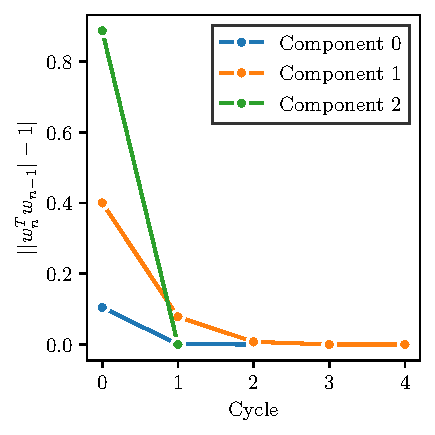
\includegraphics{scripts/ex1_dist.pdf}
\caption{\label{fig:ex1_dist} The convergence criterion $||\mathbf{w}_{n}^t \mathbf{w}_{n-1}| - 1|$ as a function of cycle for each row of $W$.}
\end{figure}
The sources predicted by the algorithm as implemented in our code and in \lstinline{sklearn.decomposition.FastICA} are shown in Fig.~\ref{fig:ex1_sources}(d, e).
Both of the results are very similar in terms of the ability to separate out independent sources.
The main difference is the sign of the sawtooth wave because independence is up to a minus sign as discussed previously in the formalism section.
From the predicted sources $\mathbf{s}_{\mathrm{predicted}}$, we can verify the accuracy of FastICA results by inverting the mixing and whitening transformations and adding back the mean of each mixture to retrieve the input signals.
\begin{align}
\mathbf{x}_{\mathrm{retrived}} &= (\mathbf{W} \mathbf{K})^{-1} \mathbf{s}_{\mathrm{predicted}} + \mathbb{E}[\mathbf{x}], \label{eq:ex1_retrieved}
\end{align}
where $\mathbf{K}$ is the whitening transformation.
The retrieved signals $\mathbf{x}_{\mathrm{retrieved}}$ are shown to be equal to the original input signals $\mathbf{x}$ (Fig.~\ref{fig:ex1_sources}(c)), which confirms that we can exactly reproduce the observed data from the output of ICA.
\begin{figure*}
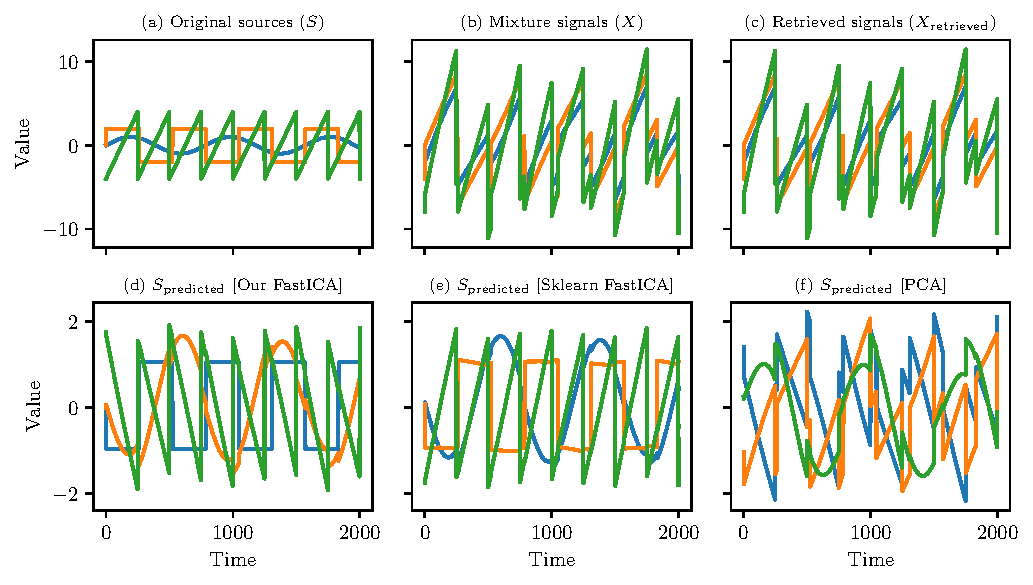
\includegraphics{scripts/ex1_sources.pdf}
\caption{\label{fig:ex1_sources}
(a) Original sources as defined in Eq.~(\ref{eq:ex1_sources}).
(b) Mixture signals whose mixing matrix is defined by Eq.~(\ref{eq:ex1_mixing}).
(c) Retrieved input signals from the predicted sources according to Eq.~(\ref{eq:ex1_retrieved}).
(d) Separated sources using our implementation of FastICA.
(e) Separated sources using \lstinline{sklearn.decomposition.FastICA}.
(f) Separated sources using \lstinline{sklearn.decomposition.PCA}.
}
\end{figure*}
In some applications, such as separation of independent sound sources, we might not need to retrieve the original mixtures.
However, this procedure becomes crucial in other applications, such as blink removals of the electroencephalogram (EEG) data. The discussion of both mentioned applications follows.

In this specific example, the result from \lstinline{sklearn.decomposition.PCA} is also plotted in Fig.~\ref{fig:ex1_sources}(f).
The figure shows that PCA is not suitable for separating independent sources.


\subsection{Application 2: audio source separation}
We employ the maximum likelihood algorithm to separate out the independent components of five mixed sound tracks~\cite{ng_cs229}.
The mixed sound waves are shown in Fig.~\ref{fig:sound} left panels (red).
The separated independent sound tracks are shown in the right panels (blue) in Fig.~\ref{fig:sound}.
The separated sound tracks can be played and listened one by one to verify that they are meaningful.
\begin{figure}[b]
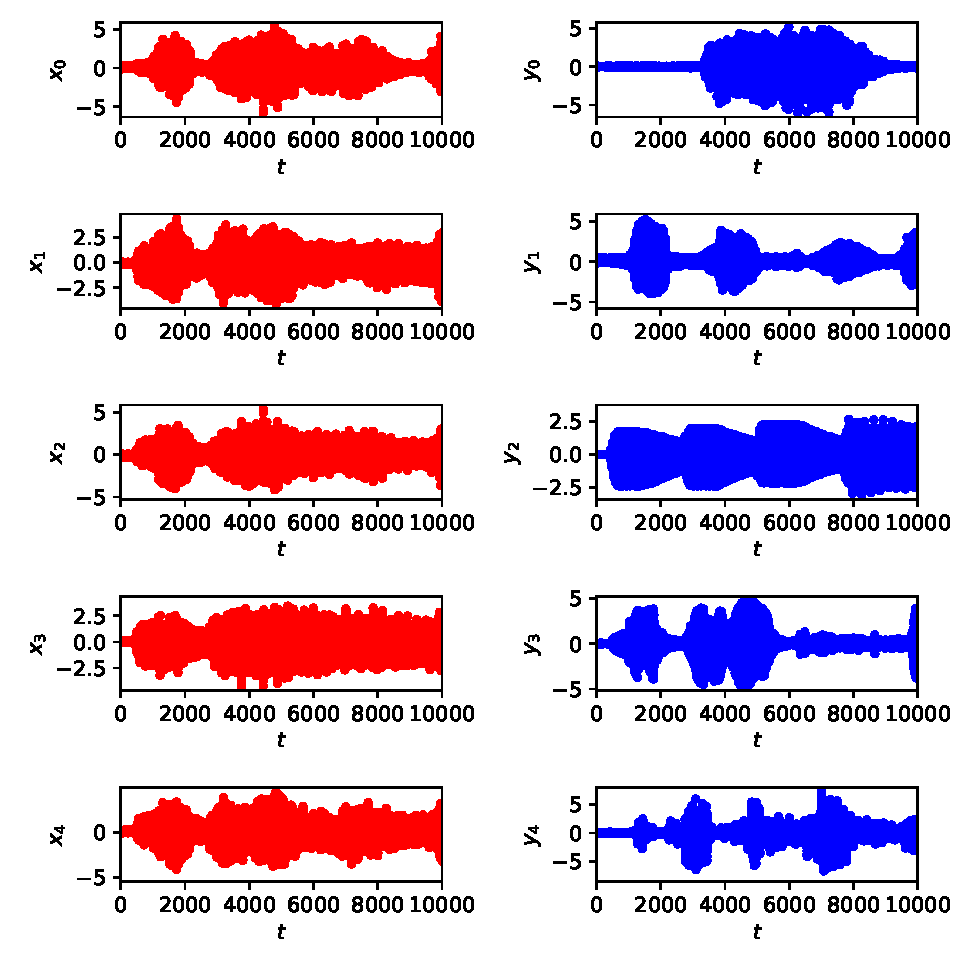
\includegraphics[width=0.8\textwidth]{scripts/sound_example.pdf}
 \caption{\label{fig:sound} shows the ICA results of separating the five mixed sound waves in the left panels (red). The separated independent components are shown in the right panels (blue). When the separated signals are played, one can clearly recognize these meaningful audio signals.}
\end{figure}

\subsection{Application 3: blinking removal in EEG signals}

In Fig.~\ref{fig:ex3_ica}, we decompose the EEG signals~\cite{talebi2021eeg} from 64 detectors into 64 independent components.
We are able to identity the 48th component to be associated with blinking signals because of the four visible peaks.
The 48th component shows a different time structure in Fig....
We reconstruct the signals $\mathbf{x}_{\mathrm{retrived}}$ using Eq.~\ref{eq:ex1_retrieved} with the 48th component set to zero.
The final result is shown in Fig.~\ref{fig:ex3_noblinks} in orange.
\begin{figure*}
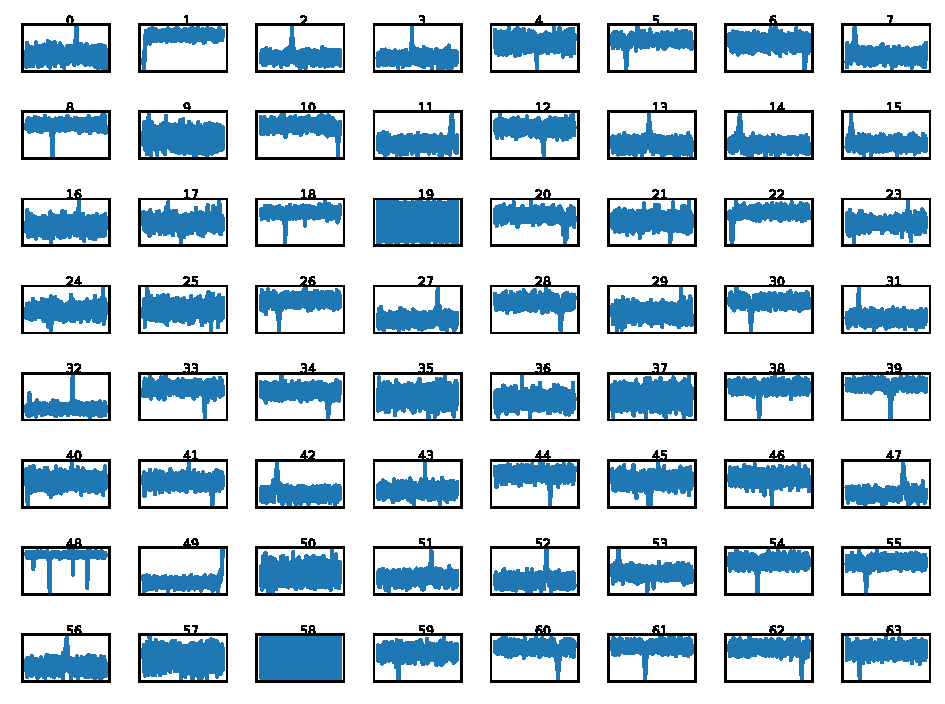
\includegraphics{scripts/ex3_ica.pdf}
\caption{\label{fig:ex3_ica} All 64 independent components separated by the moment-based algorithm.}
\end{figure*}
\begin{figure*}
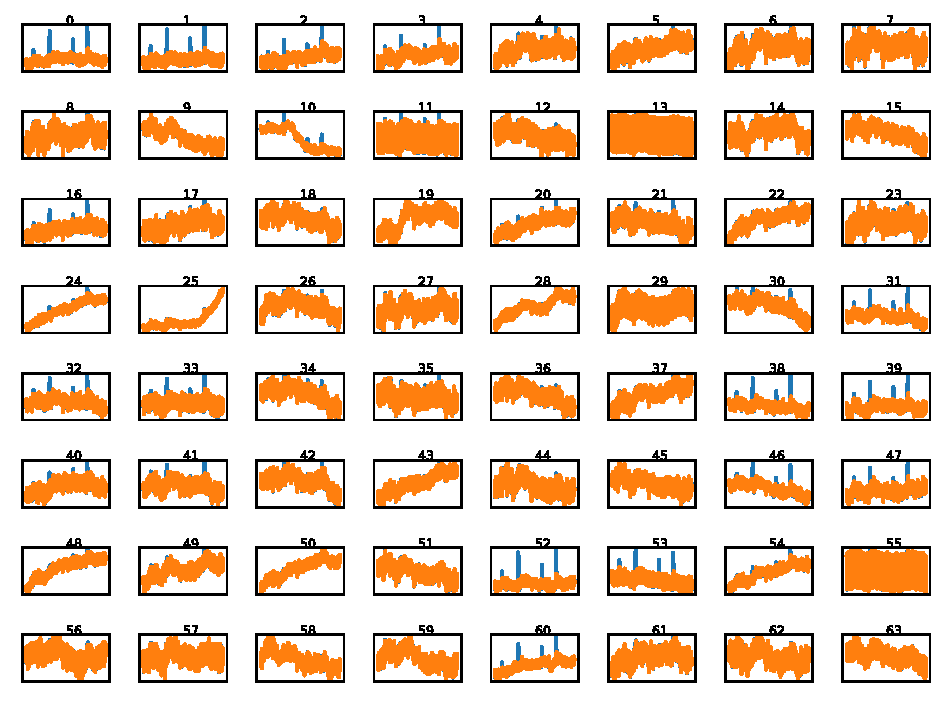
\includegraphics{scripts/ex3_noblinks.pdf}
\caption{\label{fig:ex3_noblinks} Original signals (blue) and reconstructed signals with the blinking component removed (orange).}
\end{figure*}

% (https://towardsdatascience.com/independent-component-analysis-ica-a3eba0ccec35)

%\section{How to check the robustness and convergence}
% Amari metric, ref "ELements of Statistical Learning", p.570

%1) check if the performance matrix is identity (Te-won Lee, p. 51)
%\begin{align}
%W A &= I.
%\end{align}

%2) check how fast w changes (ICA_projectionPursuit1612.05445.pdf, p. 12)

%\section{what if two of the sources are dependent}
%s3 = signal.sawtooth(2*np.pi*time) # saw tooth signal
%s4 = s1 + s2
%s5 = s1 - s2

\section{Conclusions}
In this review paper of ICA, we discuss the traditional and basic notions of this technique. We also implement the algorithms and utilize our codes in three different applications.
We notice that the objective function plays an important role in the performance of ICA in various examples we examined.
In the basic setting, the performance of the algorithm lies in choosing the correct and robust objective function.
Several objective functions have been proposed to improve the robustness and computation efficiency.
However, if we know in advance what the probability distributions look like for the sources or latent variables, it is always the best to tailor the objective function to include this information.
Nonetheless, ICA has already shown reliable performance in examples such as sound waves identification and EEG signal separation using some default robust objective functions.
The ongoing research in this field include cases where the number of detectors is smaller than the number of sources and non-linear mixing problems.

\bibliography{paper}{}

\end{document}
\grid
\grid
\grid
